% 流体力学笔记 —— 流体的物理性质
% 第 1 章：流体的物理性质

\section{流体的连续介质模型}

流体的连续介质模型具有如下性质：
\begin{enumerate}
	\item 流体是连续分布的物质，可以无限分割为具有均布质量的宏观微元体；
	\item 不发生化学反应和离解等非平衡热力学过程的运动流体中，微元体内流体状态服从热力学关系；
	\item 除特殊面（如激波）外，流体的力学和热力学状态参数在时空中是连续分布的，并且通常认为是无限可微的。
\end{enumerate}

\begin{keybox}[连续介质模型的适用条件]
	连续介质模型适用于所考察的流体的运动尺度 $L$ 远远大于流体分子运动的平均自由程 $l$ 的情况，即
	\[
	\frac{L}{l}\gg 1
	\]
\end{keybox}

上面说过，流体可以无限分割为具有均布质量的宏观微元体，这样的宏观微元体称为\textbf{流体微团}。

\begin{definition}[流体微团]
	流体微团是宏观上无限小、微观上无限大的一个质量体，其体积 $\delta V$ 满足：
	\begin{enumerate}
		\item $\dfrac{\delta V}{L^3}\ll 1$，即宏观上无限小；
		\item $\dfrac{\delta V}{l^3}\gg 1$，即微观上无限大。
	\end{enumerate}
\end{definition}

\begin{note}
	形象地说，流体微团是宏观上无限小、微观上无限大的一个质量体。（好抽象）
\end{note}

微团具有宏观无限小的体积，因此可以用时空中的一个点来标记它。连续介质的当地物性可以用时空变量 $(\boldsymbol{x},t)$ 的函数来描述，例如气体中的密度分布 $\rho=\rho(\boldsymbol{x},t)$,温度分布 $T=T(\boldsymbol{x},t)$ 等。

\begin{definition}[流体质点]
	当不需要考虑微团的体积和变形，只研究它的位移和各物理状态时，可以把它视作无体积的质点，这时称流体微团为\textbf{流体质点}。
\end{definition}

\section{作用在流体上的体积力和表面力}
在流体中任取一个微团，其上受到两种外力:第一种外力作用在微团内均布质量的质心上，这种力通常和微团的体积成正比，称为体积力:第二种外力是周围流体或物体作用在流体微团表面上的力，它和力的作用面大小成正比，称为表面力。
\begin{definition}[体积力]
	作用在微团内均布质量的质心上的外力，通常与微团的体积成正比。
\end{definition}

\begin{definition}[表面力]
	作用在微团表面上的外力，通常与力的作用面大小成正比。
\end{definition}

\subsection{体积力和体积力强度}
举两个例子。

例如，在地球引力场中，流体微团受到的引力 $\delta\boldsymbol{G}$ 与它的质量 $\delta m$ 成正比：
\begin{equation}\label{eq:gravity}
	\delta\boldsymbol{G}=\boldsymbol{g}\,\delta m
\end{equation}
式中 $\boldsymbol{g}$ 是重力加速度。由于微团的质量 $\delta m$ 与它的体积 $\delta V$ 成正比（$\delta m=\rho\,\delta V$），因此引力 $\delta\boldsymbol{G}$ 也和微团的体积成正比，它是体积力：
\begin{equation}\label{eq:gravity-volume}
	\delta\boldsymbol{G}=\boldsymbol{g}\rho\,\delta V
\end{equation}
除了引力外，还有其他形式的体积力。例如，带电质点在静电场中运动时，静电力也是一种体积力。设流体微团的电荷密度为 $q\ (\mathrm{C/m^3})$，则在静电场 $\boldsymbol{E}$ 中，该微团受到的静电力为
\begin{equation}\label{eq:electrostatic}
	\delta\boldsymbol{F}=q\,\boldsymbol{E}\,\delta V
\end{equation}

上面讲完了体积力的一些例子，理解了一下定义，下面看看怎么衡量体积力的大小。引入一个体积力强度，表达如下：
\begin{equation}\label{eq:bodyforce-intensity-def}
	\boldsymbol{f}_V=\lim_{\delta V \to 0}\frac{\delta \boldsymbol{F}}{\delta V}
\end{equation}

于是引力的体积力强度为：$\rho \boldsymbol{g}$,静电力的体积力强度为：$q \boldsymbol{E}$。

有限体积流体上所受体积力的合力，以及体积力相对于某参考点的合力矩，可以用积分方法计算。

体积力的合力：
\begin{equation}\label{eq:bodyforce-resultant}
	\boldsymbol{F}=\int_{V}\boldsymbol{f}_V d V
\end{equation}

体积力的合力矩：
\begin{equation}\label{eq:bodyforce-moment}
	\boldsymbol{L}=\int_{V}\boldsymbol{r}\times\boldsymbol{f}_V dV
\end{equation}
式中 $\boldsymbol{r}$ 为任意一流体微团相对于参考点的向径。

\subsection{表面力和应力}
任取一有限体积的流体，它的表面上受到周围流体或物体的接触力，这种力分布于有限体的表面，称为表面力，如图~\ref{fig:surfaceforce} 所示。

\begin{figure}[htbp]
	\centering
	\begin{subfigure}[b]{0.46\textwidth}
		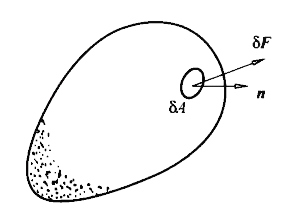
\includegraphics[width=\textwidth]{Figure/有限体上的表面力.png}
		\caption{有限体上的表面力}
	\end{subfigure}
	\hfill
	\begin{subfigure}[b]{0.46\textwidth}
		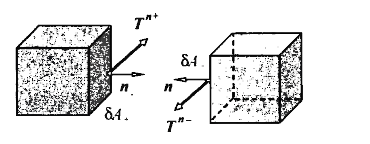
\includegraphics[width=\textwidth]{Figure/微元体上的表面力.png}
		\caption{微元体上的表面力}
	\end{subfigure}
	\caption{流体中表面力的示意图}
	\label{fig:surfaceforce}
\end{figure}

\begin{definition}[应力]
	有限体的微元面积 $\delta A$ 上单位面积的表面力称为表面力的局部强度，亦称为应力，定义如下：
	\begin{equation}\label{eq:stress-def}
		\boldsymbol{T}_n=\lim_{\delta A\to 0}\frac{\delta\boldsymbol{F}}{\delta A}
	\end{equation}
	式中 $\delta\boldsymbol{F}$ 是单位面积 $\delta A$ 上的作用力；$\boldsymbol{T}_n$ 表示应力向量，下标 $n$ 表示应力作用面 $\delta A$ 的法线方向。
\end{definition}

需要强调指出，应力与它的作用面方向有关。一般情况下，流体内部同一空间点处、不同方向的作用面上，流体所受应力是不等的，所以必须标注应力作用面的法向量。约定作用面的法向量以指向域外为正。例如图~\ref{fig:surfaceforce}(b) 中，$\delta A_{1}$ 面的法向量为 $\boldsymbol{n}_{A_{+}}$，作用在其上的应力为 $\boldsymbol{T}_{n_{A_{+}}}$；相邻面 $\delta A$ 的法向量为 $\boldsymbol{n}_{A_{-}}$，其上应力符号为 $\boldsymbol{T}_{n_{A_{-}}}$。

应力 $\boldsymbol{T}_n$ 是向量，一般情况下它并不垂直于它的作用面，所以可将其分解为垂直于作用面的分量 $T_{nn}$ 和平行于作用面的两个相互垂直分量 $T_{ns}$ 和 $T_{nt}$。约定 $(\boldsymbol{n},\boldsymbol{t},\boldsymbol{s})$ 组成右手直角坐标系。根据上述约定，应力分量的第一个下标表示应力作用面的法向，第二个下标表示应力分量的方向。

\begin{definition}[正应力]
	应力向量在作用面法线方向的分量称为正应力。根据应力分量的约定，正值的正应力指向作用面外，是拉力；负值的正应力指向作用面内，因而是压力。依旧和材料力学里一样使用"拉正压负"的约定。
\end{definition}

\begin{definition}[切应力]
	应力向量在作用面切向的分量称为切应力，也称剪应力。
\end{definition}

\begin{property}
	应力具有以下性质：
	\begin{enumerate}
		\item 相邻两微元面上的表面力是作用力与反作用力，因此它们大小相等、方向相反。令 $n_A=-n$，则 $\boldsymbol{T}_{-n}=-\boldsymbol{T}_n$，即
		\[
			\boldsymbol{T}_{-n}=\lim_{\delta A\to 0}\frac{-\delta\boldsymbol{F}}{\delta A}=-\boldsymbol{T}_n
		\]
		\item 相邻微元面上的正应力和切应力值都相等。
	\end{enumerate}
\end{property}

\begin{proof}
	在 $\delta A_n$ 面上的正应力 $T_{nn}$ 等于
	\begin{equation}\label{eq:normal-stress}
		T_{nn}=\boldsymbol{T}_n\cdot\boldsymbol{n}
	\end{equation}
	相邻面 $\delta A$ 上正应力为 $T_{-n,-n}=\boldsymbol{T}_{-n}\cdot(-\boldsymbol{n})$。利用相邻面上的应力关系，很容易证明相邻面上的正应力相等：
	\begin{equation}\label{eq:normal-stress-equal}
		T_{-n,-n}=\boldsymbol{T}_{-n}\cdot(-\boldsymbol{n})=(-\boldsymbol{T}_n)\cdot(-\boldsymbol{n})=\boldsymbol{T}_n\cdot\boldsymbol{n}=T_{nn}
	\end{equation}

	在 $\delta A_n$ 面上的切应力等于
	\begin{equation}\label{eq:shear-stress}
		\left\{\begin{array}{l}
			T_{nt}=\boldsymbol{T}_n\cdot\boldsymbol{t}\\
			T_{ns}=\boldsymbol{T}_n\cdot\boldsymbol{s}
		\end{array}\right.
	\end{equation}
	在相邻面 $\delta A$ 上相应的切应力分量为 $T_{-n,-t}$、$T_{-n,-s}$。同理可证两相邻面上的切应力分量也相等：
	\begin{equation}\label{eq:shear-stress-equal}
		\left\{\begin{array}{l}
			T_{-n,-t}=\boldsymbol{T}_{-n}\cdot(-\boldsymbol{t})=(-\boldsymbol{T}_n)\cdot(-\boldsymbol{t})=\boldsymbol{T}_n\cdot\boldsymbol{t}=T_{nt}\\
			T_{-n,-s}=\boldsymbol{T}_{-n}\cdot(-\boldsymbol{s})=(-\boldsymbol{T}_n)\cdot(-\boldsymbol{s})=\boldsymbol{T}_n\cdot\boldsymbol{s}=T_{ns}
		\end{array}\right.
	\end{equation}
\end{proof}

\subsection{一点的应力张量及其性质}

\begin{definition}[一点的应力状态]
	通过同一点不同面上的应力一般不相等，但只要知道通过一点三个互相垂直坐标面上的应力值，就可以确定该点任意方向面上的应力。因此称这三个互相垂直面上的应力 $(\boldsymbol{T}_1,\boldsymbol{T}_2,\boldsymbol{T}_3)$ 为一点的应力状态。
\end{definition}

众所周知，一个向量可以分解为三个分量（其实几个分量都行，这里讨论应力状态），因此每个应力向量 $\{\boldsymbol{T}_i\}$ 都可以分解为三个分量如下：
\begin{equation}\label{eq:stress-decompose}
	\left\{\begin{array}{l}
		\boldsymbol{T}_1=T_{11}\boldsymbol{e}_1+T_{12}\boldsymbol{e}_2+T_{13}\boldsymbol{e}_3\\
		\boldsymbol{T}_2=T_{21}\boldsymbol{e}_1+T_{22}\boldsymbol{e}_2+T_{23}\boldsymbol{e}_3\\
		\boldsymbol{T}_3=T_{31}\boldsymbol{e}_1+T_{32}\boldsymbol{e}_2+T_{33}\boldsymbol{e}_3
	\end{array}\right.
\end{equation}
于是一点应力状态还可以用九个代数值组成的方阵表示：
\begin{equation}\label{eq:stress-tensor}
	[T_{ij}]=\begin{bmatrix}
		T_{11} & T_{12} & T_{13}\\
		T_{21} & T_{22} & T_{23}\\
		T_{31} & T_{32} & T_{33}
	\end{bmatrix}
\end{equation}

\begin{definition}[应力张量]
	任意面上的应力可写作
	\begin{equation}\label{eq:stress-tensor-action}
		\boldsymbol{T}_n=\boldsymbol{T}_i\,n_i=T_{ij}\boldsymbol{e}_j\,n_i
	\end{equation}
	利用\textbf{张量识别定理}可以证明一点应力状态是张量，因而 $T_{ij}$ 称为应力张量的分量，$[T_{ij}]$ 称为应力张量。
\end{definition}

\begin{property}[一点应力张量的确定]
	过一点任意面上的应力 $\boldsymbol{T}_n$，由通过该点三个相互垂直面上的应力 $(\boldsymbol{T}_1,\boldsymbol{T}_2,\boldsymbol{T}_3)$ 完全确定，即
	\begin{equation}\label{eq:stress-arbitrary}
		\boldsymbol{T}_n=\boldsymbol{T}_1\,n_1+\boldsymbol{T}_2\,n_2+\boldsymbol{T}_3\,n_3=\boldsymbol{T}_i\,n_i
	\end{equation}
	因此，一点的应力状态可用九个分量 $T_{ij}$（即应力张量）完全描述。
\end{property}

\begin{proof}
	为了论述简明起见，在点 $O$ 处取一直角四面体（如图~\ref{fig:stressstate}），其中三个面为坐标面，任意倾斜面具有法向量 $\boldsymbol{n}$ 和面积 $\delta A_n$。

	\begin{figure}[htbp]
		\centering
		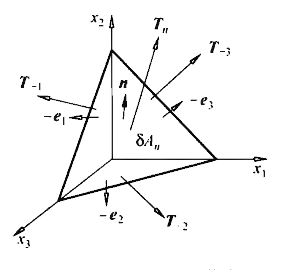
\includegraphics[width=0.5\textwidth]{Figure/一点的应力状态.png}
		\caption{一点的应力状态}
		\label{fig:stressstate}
	\end{figure}

	图~\ref{fig:stressstate} 中四面体四个面上的法向量分别为 $\boldsymbol{n}$、$-\boldsymbol{e}_1$、$-\boldsymbol{e}_2$、$-\boldsymbol{e}_3$；作用的应力分别为 $\boldsymbol{T}_n$、$\boldsymbol{T}_1$、$\boldsymbol{T}_2$、$\boldsymbol{T}_3$；直角四面体的四个表面积分别为 $\delta A_n$、$\delta A_1$、$\delta A_2$、$\delta A_3$。根据面积投影定理，$\delta A_i\ (i=1,2,3)$ 与 $\delta A_n$ 的关系为
	\begin{equation}\label{eq:area-projection}
		\delta A_i=\delta A_n\,n_i
	\end{equation}

	现在我们来建立该微元四面体的力学平衡式。假定微元体处于体积力强度 $\rho\boldsymbol{f}$ 的外力场中，则按牛顿定律 $F=ma$（$m=\rho\,\delta V$ 是微元体的质量，$\boldsymbol{a}$ 是微团加速度），四面体的平衡方程应为
	\begin{equation}\label{eq:tetrahedron-eq}
		\rho\boldsymbol{a}\,\delta V=\rho\boldsymbol{f}\,\delta V+\boldsymbol{T}_n\,\delta A_n+\boldsymbol{T}_{-1}\,\delta A_1+\boldsymbol{T}_{-2}\,\delta A_2+\boldsymbol{T}_{-3}\,\delta A_3
	\end{equation}
	式中 $\delta V$ 是微元体的体积。方程左端为微元体的质量与加速度的乘积，右端第一项是作用在四面体上的体积力的合力，右端后四项是作用在四面体表面上的表面力的合力。将等式两边同除以 $\delta A_n$，则明显有
	\begin{equation}
		\lim_{\delta A_n\to 0}\frac{\delta V}{\delta A_n}=0
	\end{equation}
	此外，由面积投影关系 $\dfrac{\delta A_i}{\delta A_n}=n_i$，因而有
	\begin{equation}
		\boldsymbol{T}_n+\boldsymbol{T}_{-1}\,n_1+\boldsymbol{T}_{-2}\,n_2+\boldsymbol{T}_{-3}\,n_3=0
	\end{equation}
	注意到相邻面上应力关系 $\boldsymbol{T}_{-i}=-\boldsymbol{T}_i$，上式可写作（使用爱因斯坦求和约定），即得式~\eqref{eq:stress-arbitrary}。
\end{proof}

\subsection{应力张量的对称性}
\begin{property}[应力张量的对称性]
	由微团的力矩平衡原理，可以进一步证明，九个应力分量不是相互独立的，而有以下的对称关系式
	\begin{equation}\label{eq:stress-symmetry}
		T_{ij}=T_{ji}
	\end{equation}
	即应力分量的方阵是对称方阵，或者说应力张量是对称张量。因此，连续介质中一点的应力张量只有六个独立分量。
\end{property}

\begin{proof}[应力张量对称性的证明]
	根据动量矩定理：有限质量体的动量矩增长率等于作用在该质量体上的外力矩之和。在流体中取任意一有限体积流体，作用在该有限体表面 $\Sigma$ 上的外力矩为
	\begin{equation}
		\boldsymbol{L}_\Sigma=\oiint_\Sigma \boldsymbol{r}\times\boldsymbol{T}_n\,\mathrm{d}A=\oiint_\Sigma \boldsymbol{r}\times T_{ni}\boldsymbol{e}_i\,\mathrm{d}A
	\end{equation}
	体积力矩为
	\begin{equation}
		\boldsymbol{L}_V=\iiint_V \rho\,(\boldsymbol{r}\times\boldsymbol{f})\,\mathrm{d}V
	\end{equation}
	有限体的动量矩用 $\boldsymbol{K}$ 表示，它的增长率为
	\begin{equation}
		\frac{\mathrm{d}\boldsymbol{K}}{\mathrm{d}t}=\iiint_V \rho\,(\boldsymbol{r}\times\boldsymbol{a})\,\mathrm{d}V
	\end{equation}
	根据动量矩原理 $\dfrac{\mathrm{d}\boldsymbol{K}}{\mathrm{d}t}=\boldsymbol{L}_\Sigma+\boldsymbol{L}_V$，应有
	\begin{equation}
		\iiint_V \rho\,(\boldsymbol{r}\times\boldsymbol{a})\,\mathrm{d}V=\oiint_\Sigma \boldsymbol{r}\times T_{ni}\boldsymbol{e}_i\,\mathrm{d}A+\iiint_V \rho\,\boldsymbol{r}\times\boldsymbol{f}\,\mathrm{d}V
	\end{equation}
	式中面积分可以用高斯公式（见附录）转换成体积分：
	\begin{equation}
		\oiint_\Sigma \boldsymbol{r}\times\boldsymbol{T}_i\,n_i\,\mathrm{d}A=\iiint_V \frac{\partial}{\partial x_i}(\boldsymbol{r}\times\boldsymbol{T}_i)\,\mathrm{d}V
	\end{equation}
	体积分中的被积函数可以进一步化简：
	\begin{equation}
		\frac{\partial}{\partial x_i}(\boldsymbol{r}\times\boldsymbol{T}_i)=\frac{\partial\boldsymbol{r}}{\partial x_i}\times\boldsymbol{T}_i+\boldsymbol{r}\times\frac{\partial\boldsymbol{T}_i}{\partial x_i}
	\end{equation}
	向量 $\boldsymbol{r}=x_1\boldsymbol{e}_1+x_2\boldsymbol{e}_2+x_3\boldsymbol{e}_3=x_i\boldsymbol{e}_i$，故被积函数为
	\begin{equation}
		\frac{\partial}{\partial x_i}(\boldsymbol{r}\times\boldsymbol{T}_i)=\boldsymbol{e}_i\times\boldsymbol{T}_i+\boldsymbol{r}\times\frac{\partial\boldsymbol{T}_i}{\partial x_i}
	\end{equation}
	将它代入动量矩定理表达式后，得
	\begin{equation}
		\iiint_V\left(\boldsymbol{e}_i\times\boldsymbol{T}_i+\boldsymbol{r}\times\frac{\partial\boldsymbol{T}_i}{\partial x_i}+\rho\,\boldsymbol{r}\times\boldsymbol{f}-\rho\,\boldsymbol{r}\times\boldsymbol{a}\right)\mathrm{d}V=0
	\end{equation}
	将有限体积无限缩小，这时被积函数中位置向量 $|\boldsymbol{r}|\to 0$，因而被积函数中后三项较第一项小一个量级；当取极限 $V\to 0$ 时，后三项可略去不计。于是微团的动量矩定理表达式简化为
	\begin{equation}
		\boldsymbol{e}_i\times\boldsymbol{T}_i=0
	\end{equation}
	用应力张量的分量表示 $\boldsymbol{T}_i=T_{ij}\boldsymbol{e}_j$，上式可写为
	\begin{equation}
		\boldsymbol{e}_i\times\boldsymbol{T}_i=\boldsymbol{e}_i\times T_{ij}\boldsymbol{e}_j=T_{ij}(\boldsymbol{e}_i\times\boldsymbol{e}_j)
	\end{equation}
	在向量运算中（见附录）有以下公式
	\begin{equation}
		\boldsymbol{e}_i\times\boldsymbol{e}_j=-\boldsymbol{e}_j\times\boldsymbol{e}_i
	\end{equation}
	代入前式并交换哑指标，得
	\begin{equation}
		T_{ij}(\boldsymbol{e}_i\times\boldsymbol{e}_j)=-T_{ij}(\boldsymbol{e}_j\times\boldsymbol{e}_i)=-T_{ji}(\boldsymbol{e}_i\times\boldsymbol{e}_j)
	\end{equation}
	于是有
	\begin{equation}
		(T_{ij}-T_{ji})(\boldsymbol{e}_i\times\boldsymbol{e}_j)=0
	\end{equation}
	由于 $\boldsymbol{e}_i\times\boldsymbol{e}_j$ 不全为零，故
	\begin{equation}
		T_{ij}=T_{ji}
	\end{equation}
\end{proof}

\subsection{理想流体的应力张量}
\begin{theorem}[理想流体的应力张量]
	一般来说，运动流体中的应力状态有六个分量。一种最简单的流体模型称为理想流体，这种流体中任意一点的应力状态是各向同性张量，即理想流体中任意一点的应力张量可表示为
	\begin{equation}\label{eq:ideal-fluid-stress}
		T_{ij}=-p\,\delta_{ij}
	\end{equation}
	其中 $p$ 是标量且通常大于零，负号表示正应力作用方向与作用面的外法线方向相反；$\delta_{ij}$ 是单位张量（Kronecker 符号），即
	\begin{equation}\label{eq:kronecker-delta}
		\delta_{ij}=\begin{cases}1,& i=j\\ 0,& i\neq j\end{cases}
	\end{equation}
\end{theorem}

上式表明，理想流体中任意面上只有正应力，并且就是压强 $p$，即任意面上的正应力 $T_{nn}=-p$。很容易由上述关系导出这一结论。任意面上的应力可写作式~\eqref{eq:stress-tensor-action}，因 $T_{ij}=-p\,\delta_{ij}$，故 $T_{ij}\boldsymbol{e}_j=-p\,\delta_{ij}\boldsymbol{e}_j=-p\,\boldsymbol{e}_i$，于是任意面上的应力
\begin{equation}\label{eq:ideal-fluid-stress-n}
	\boldsymbol{T}_n=-p\,\boldsymbol{e}_i\,n_i=-p\,\boldsymbol{n}
\end{equation}
上式表明任意面上的应力为正应力，同时说明任意面上的应力分量都等于 $-p$，即理想流体微团表面承受均匀分布的压强。

\section{流体的粘性和压缩性}
流体和固体的基本区别在于它的易流性。固体在剪切力作用下发生剪切变形后可以达到新的静平衡状态，而静止流体不能承受剪切力，任何微小的剪切力都能驱使流体持续流动。也就是说，静止流体中的应力只有压强，而当流体运动时，流体微团的表面除了压强外还有剪应力。流体运动时，微团之间具有抵抗相互滑移运动的属性，称为流体的粘性。
